
\newlength\cmsFigWidth
\newlength\cmsTabSkip\setlength{\cmsTabSkip}{1.7ex}
\ifthenelse{\boolean{cms@external}}{\setlength\cmsFigWidth{0.85\columnwidth}}{\setlength\cmsFigWidth{0.4\textwidth}}
\ifthenelse{\boolean{cms@external}}{\providecommand{\cmsTable}[1]{#1}}{\providecommand{\cmsTable}[1]{\resizebox{\textwidth}{!}{#1}}}
\newcommand{\mll}{m_{\ell\ell}}
\newcommand{\mjj}{m_\mathrm{jj}}
\newcommand{\mzg}{m_{\PZ\gamma}}
\newcommand{\mllg}{m_{\ell\ell\gamma}}
\newcommand{\etajj}{\abs{\Delta \eta_{\mathrm{jj}}}}
\newcommand{\gbarrel}{\gamma_{\text{barrel}}}
\newcommand{\gendcap}{\gamma_{\text{endcap}}}
\newcommand{\dphizgjj}{\Delta \phi_{\PZ\gamma,\mathrm{jj}}}
\newcommand{\mTH}{\ensuremath{\mT^{\PH}}\xspace}
\newcommand{\mTltwo}{\ensuremath{\mT^{\ell_{2}}}\xspace}
\newcommand{\ptvecll}{\ensuremath{\ptvec^{\ell\ell}}\xspace}
\newcommand{\ptll}{\ensuremath{\pt^{\ell\ell}}\xspace}
\newcommand{\dphill}{\ensuremath{\Delta\phi_{\ell\ell}}\xspace}
\newcommand{\drll}{\ensuremath{\Delta R_{\ell\ell}}\xspace}
\newcommand{\ptltwo}{\ensuremath{\pt^{\elll_{2}}}\xspace}
\newcommand{\ptvecltwo}{\ensuremath{\ptvec^{\ell_{2}}}\xspace}
\newcommand{\ttst}{\ensuremath{\ttbar\gamma{}+{}\PQt\PW}\xspace}
\newcommand{\tautau}{\ensuremath{\PGtp{}\PGtm}\xspace}

\cmsNoteHeader{SMP-22-006}

\title{Observation of $\PW\PW\gamma$ production and constraints on Higgs couplings to light quarks in proton-proton collisions at \texorpdfstring{$\sqrt{s}=13\TeV$}{sqrt(s) = 13 TeV}}

\address[cern]{CERN}
\author[cern]{The CMS Collaboration}

\date{\today}

\abstract{he first observation of $\PW\PW\gamma$ production with leptonic final states in proton-proton collisions at a center-of-mass energy of 13\TeV is presented. A data set corresponding to an integrated luminosity of 138\fbinv collected by the CMS experiment at the LHC in 2016--2018 is used. Events are selected by requiring exactly two leptons (one electron and one muon) of opposite charge, moderate missing transverse momentum, and a photon. The measured fiducial cross section for $\PW\PW\gamma$ is $\sigma = 6.04 \pm 1.69 \unit{fb}$, in good agreement with the next-to-leading order QCD prediction. The analysis is also extended to search for the associated production of a Higgs boson and a photon where the Higgs decays to $\PW^{+}\PW^{-}$, which is sensitive to the Higgs coupling with light quarks (the \PQc, \PQs, \PQu, and \PQd quarks) and a set of limits on these couplings are reported at 95\% confidence level.}

\hypersetup{
pdfauthor={Ying An, Zhe guan, Andrew Michael Levin, Qiang Li, Meng Lu, Sen Deng, Jie Xiao, Sitian Qian, Jing Peng, Congqiao Li, Qilong Guo},
pdftitle={Measurement of the triboson WWgamma production in proton-proton collisions at sqrt(s) = 13 TeV and constraints of couplings on anomalous quartic gauge and Higgs to the light quarks},
pdfsubject={CMS},
pdfkeywords={CMS,  multi-boson, Yukawa couplings}}

\maketitle 

Measurements of multiple bosons produced simultaneously are key to testing the electroweak sector of the standard model (SM). The non-abelian nature of the electroweak interaction predicts the presence of self-interacting vector boson vertices leading to a rich variety of multiboson production mechanisms. Many multiboson processes are only accessible at the LHC due to its high collision energy and the large amount of data it has collected. The CMS and ATLAS collaborations have both recently observed the production of three massive gauge bosons~\cite{CMS:2020hjs,ATLAS:2021atz}.  Production of $\PW\Pgg\Pgg$ and $\PZ\Pgg\Pgg$ have also been measured by both the ATLAS and CMS collaborations, with signal significances of at least 3 standard deviations~\cite{ATLAS:2015ify,ATLAS:2016qjc,CMS:2017tzy,CMS:2021jji}. Measurements of $\PW\PW\gamma$ have also been performed by both the CMS and ATLAS collaborations at a center-of-mass energy of 8\TeV~\cite{CMS:2014cdf,ATLAS:2017bon}, but only upper limits on the production cross sections are reported therein due to a lack of statistical power and sensitivity.

Triboson production is sensitive to both triple and quartic gauge couplings (TGCs and QGCs). The measurement of possible deviations from the theoretical predictions could provide indirect evidence of new particles or new interactions. The same final states can also be exploited to probe Higgs couplings with light quarks, \PQc, \PQs, \PQu, and \PQd, as proposed in recent literature~\cite{Khanpour:2017inb,Aguilar-Saavedra:2020rgo,Falkowski:2020znk}. As the leading order (LO) gluon-initiated contribution $gg\rightarrow h\gamma$ vanishes due to Furry’s theorem, the inclusive $h\gamma$ production at the LHC is directly related to Higgs Yukawa coupling with the light quarks. Recently, ATLAS provides a bound on the charm Yukawa coupling modifier $\kappa_c<8.5$ at 95\% confidence level~\cite{ATLAS:2021zwx}, while the upper bound on the strange Yukawa coupling is quite loose~\cite{Duarte-Campderros:2018ouv,ATLAS:2018xfc}.

At leading order in quantum chromodynamics (QCD), $\Pe^+\nu_{\Pe}\mu^-\overline{\nu}_{\mu}\Pgg$ and $\mu^+\nu_{\mu}\Pe^-\overline{\nu}_{\Pe}\Pgg$ production in $\Pp\Pp$ collisions can proceed through initial-state radiation (ISR) from one of the incoming quarks, final-state radiation (FSR) from the outgoing charged leptons, the $\PW\PW\Pgg$ TGC, the $\PW\PW\PZ\Pgg$ or $\PW\PW\Pgg\Pgg$ QGC vertices, and  associated production of a Higgs boson and a photon. Example diagrams are shown in Fig.~\ref{fig:LO diagrams}. At higher orders in QCD~\cite{Zhu:2020ous}, additional quarks can appear in the final state, and the photon can arise by FSR from an outgoing quark or lepton. 

\begin{figure*}[htp]
    \centering
    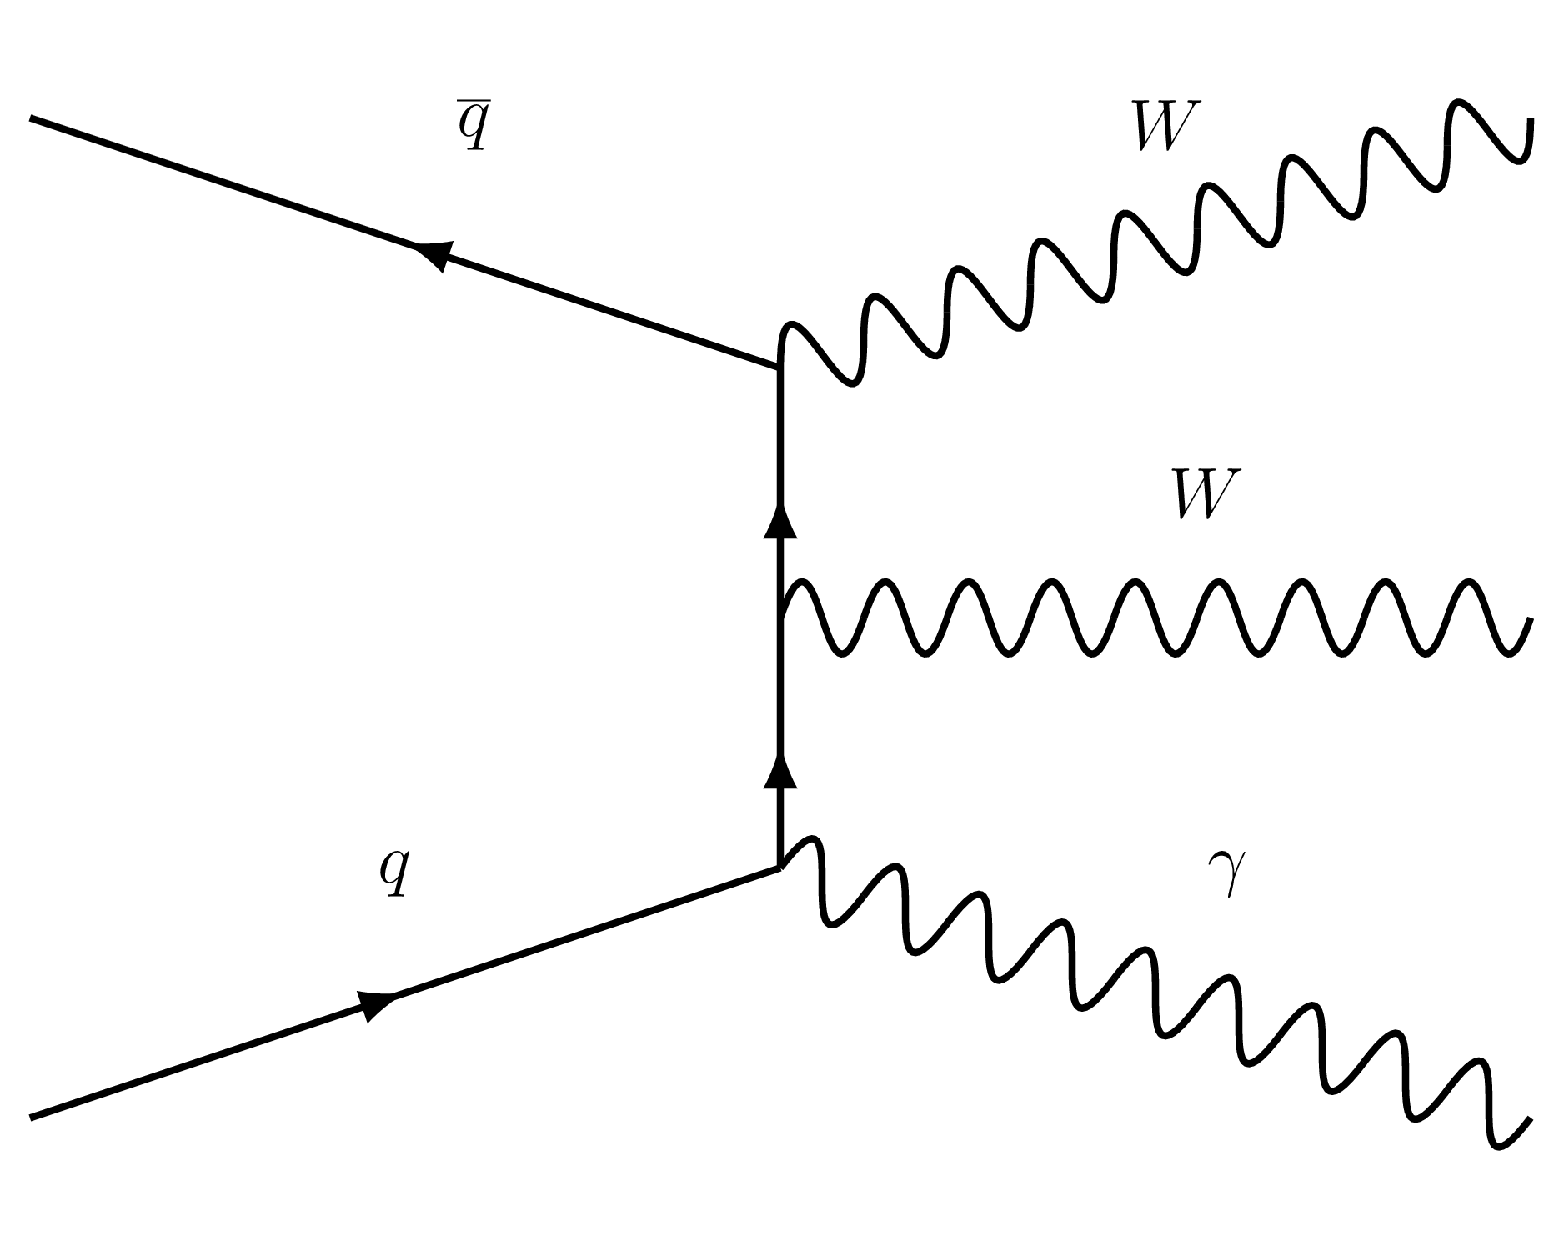
\includegraphics[width=0.22\textwidth]{ISR.pdf}
    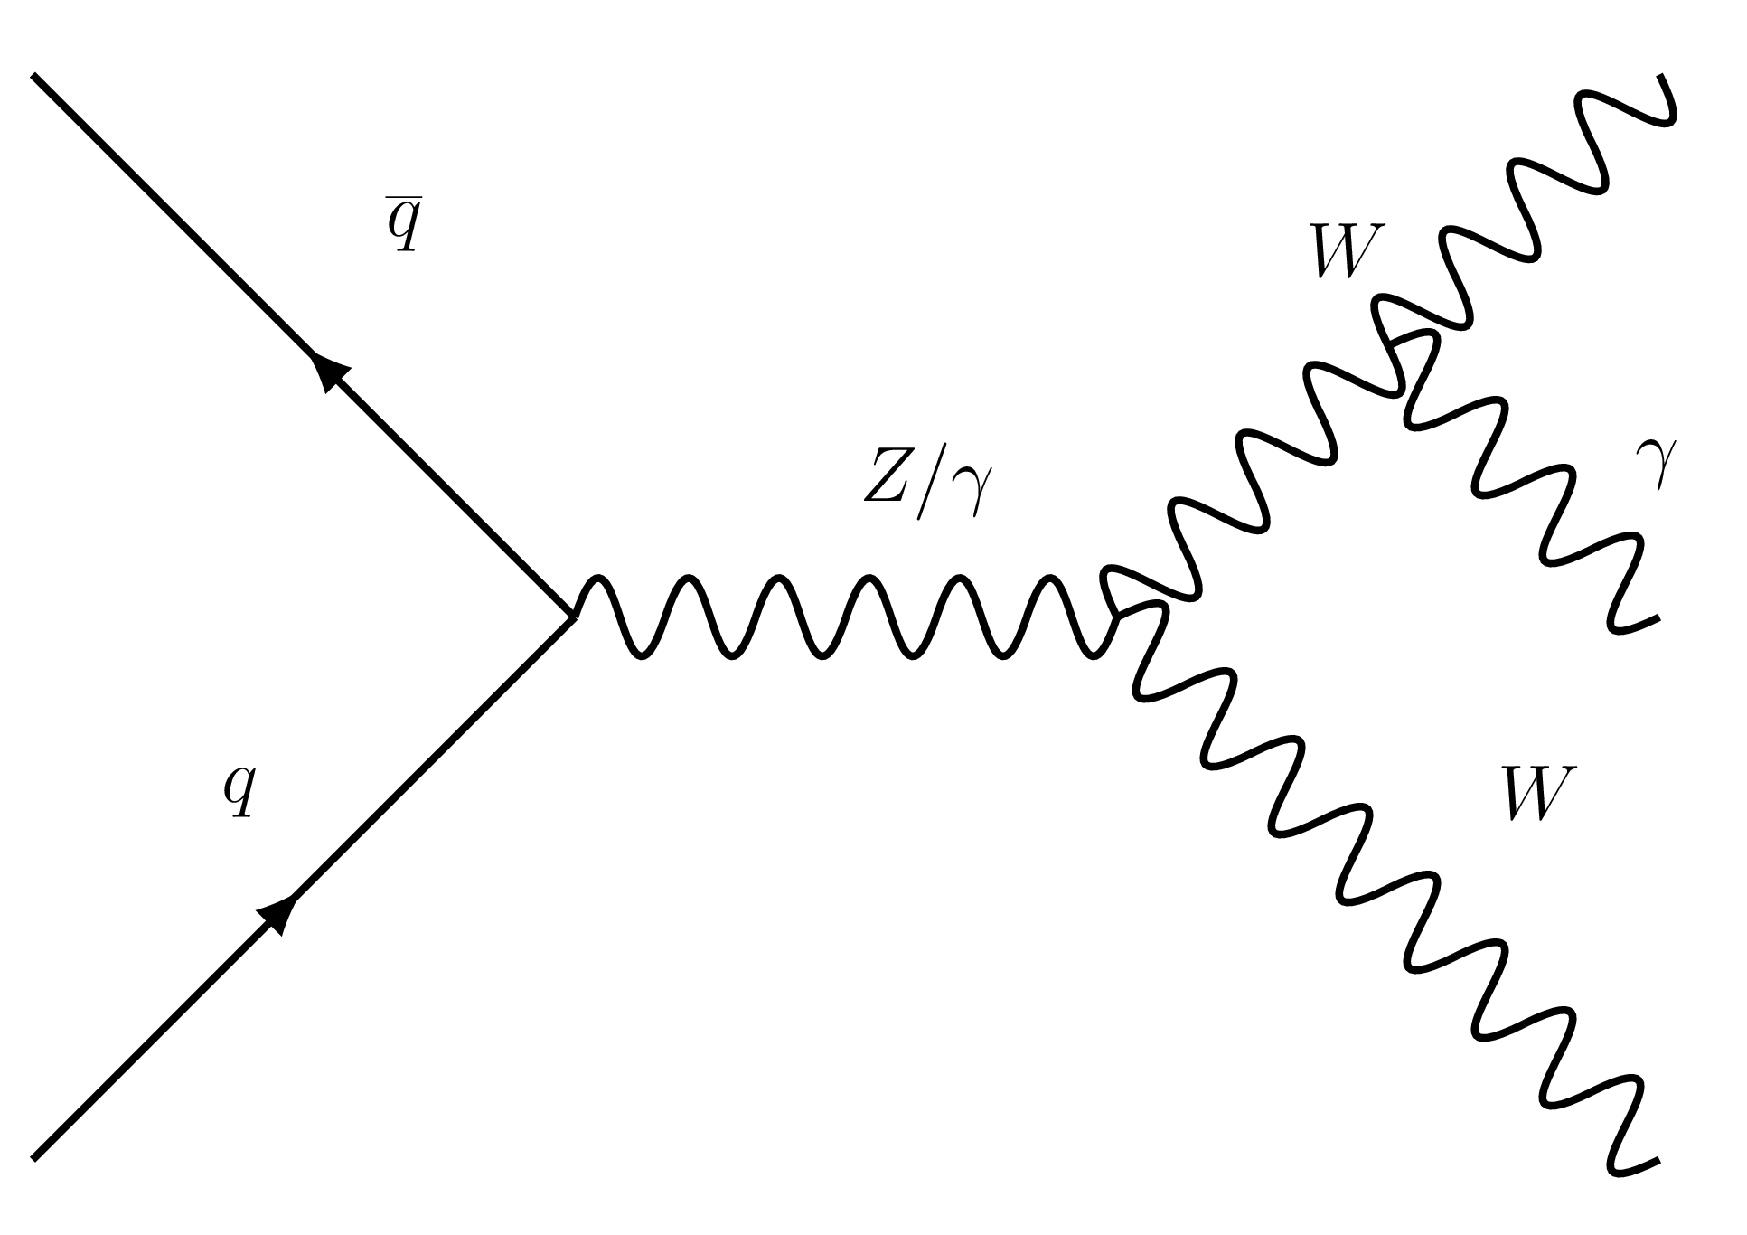
\includegraphics[width=0.22\textwidth]{FSR.pdf}
    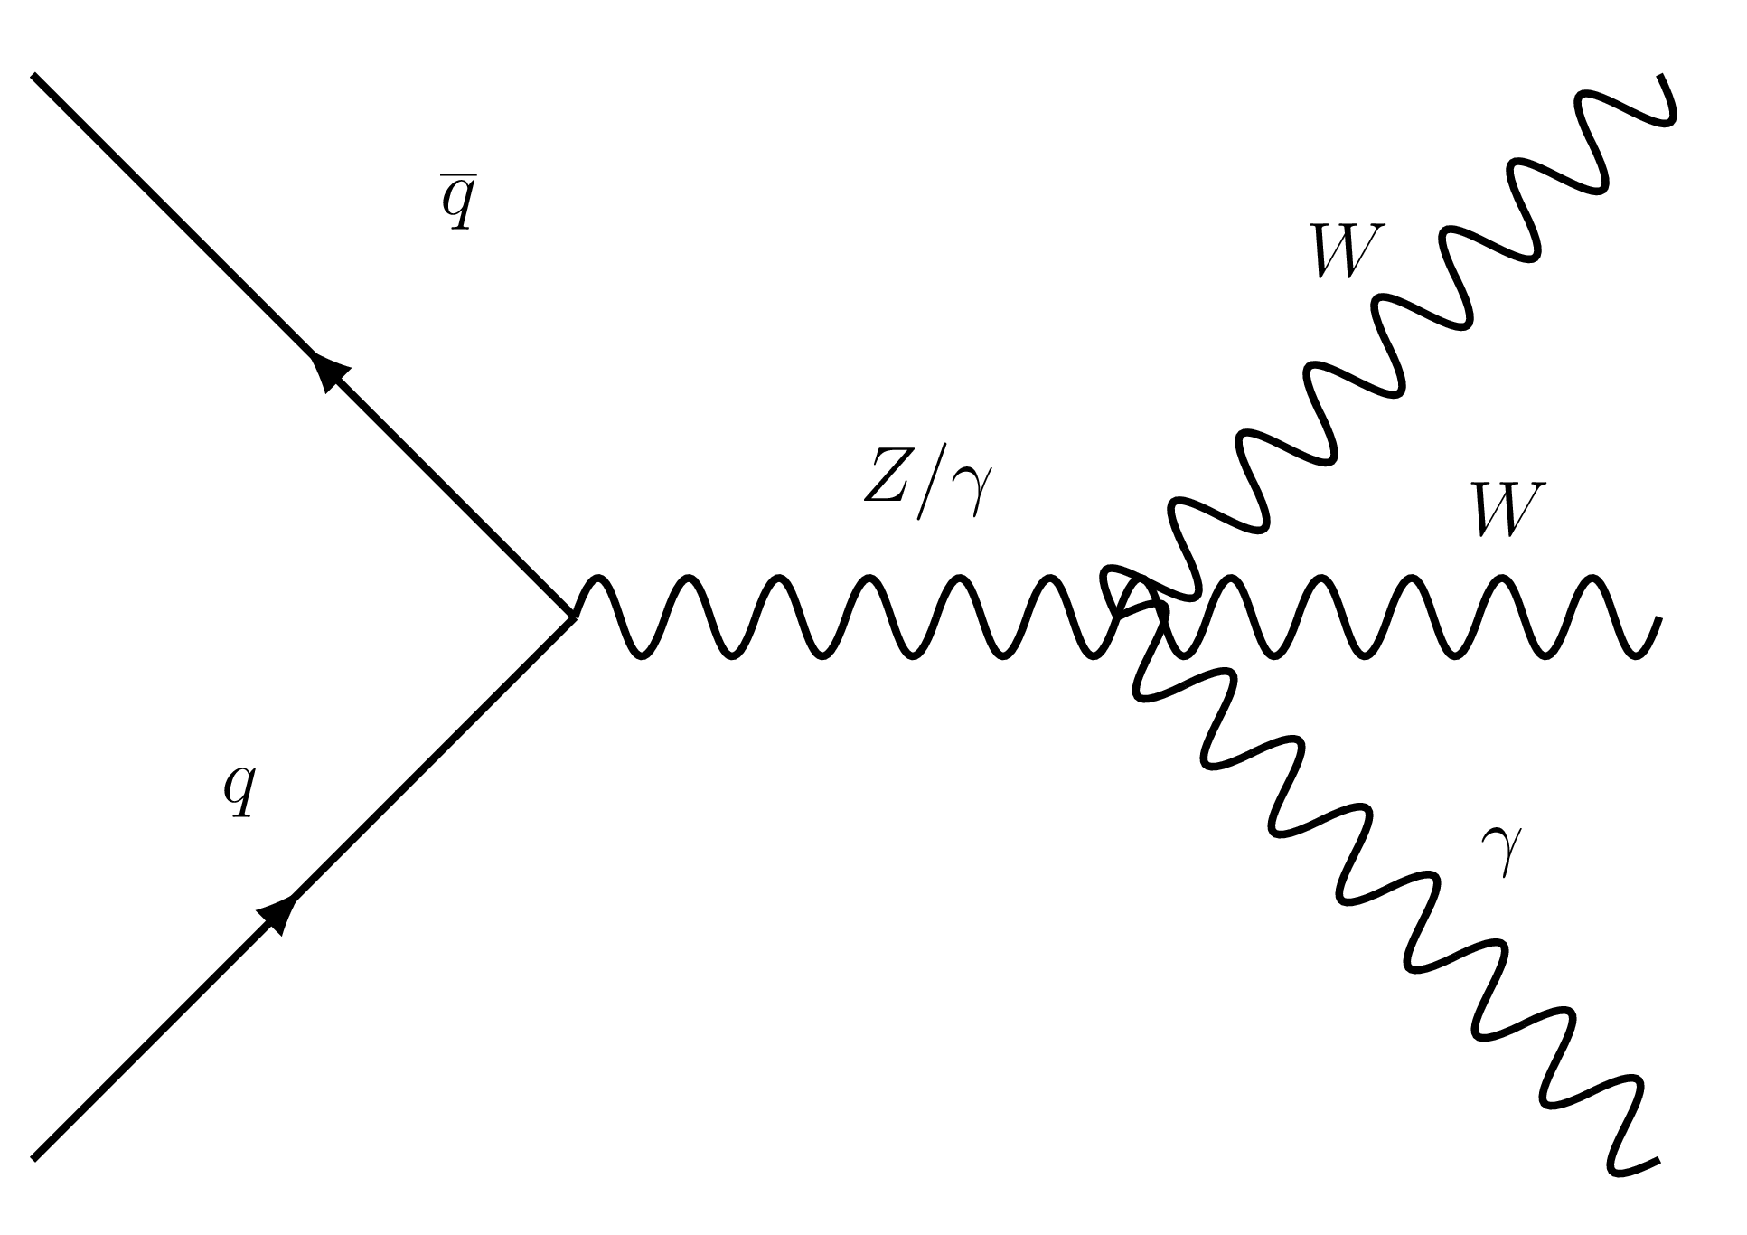
\includegraphics[width=0.22\textwidth]{aQGC.pdf}
    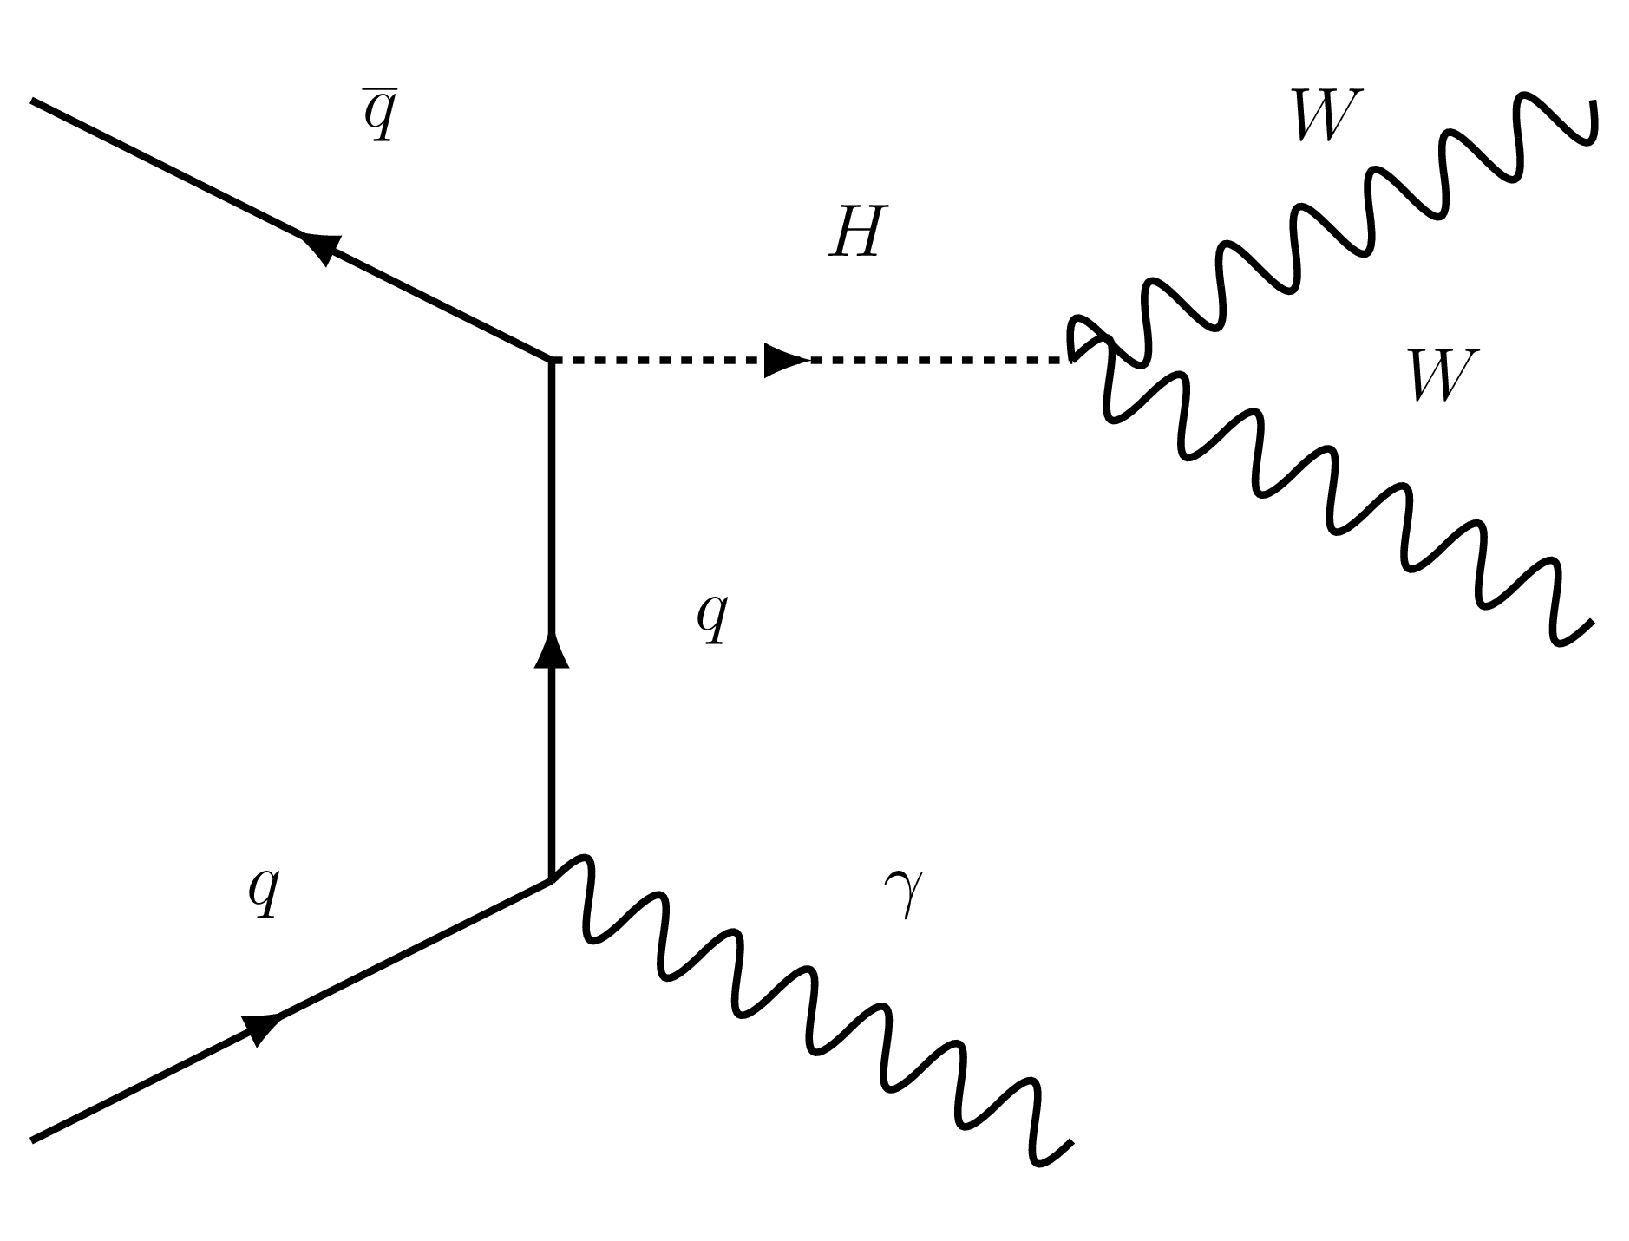
\includegraphics[width=0.22\textwidth]{HG.pdf}
    \caption{Representative Feynman diagrams for the $\PW\PW\gamma$ process. From left to right, ISR, FSR, QGC, and Higgs associated production.}
    \label{fig:LO diagrams}
\end{figure*}

This letter reports the first observation of $\PW\PW\gamma$ production along with a study of the Higgs couplings to light quarks. The measurement is based on the $\sqrt{s} = 13\TeV$ proton-proton collision data collected by the CMS detector during 2016--2018, corresponding to an integrated luminosity of $138\fbinv$.

The central feature of the CMS apparatus is a superconducting solenoid of 6\unit{m} internal diameter, providing a magnetic field of 3.8\unit{T}. Within the solenoid volume, there are a silicon pixel, a strip tracker, a lead tungstate crystal electromagnetic calorimeter, and a brass and scintillator hadron calorimeter, each composed of a barrel and two endcap sections. Forward calorimeters extend the pseudorapidity ($\eta$) coverage provided by the barrel and endcap detectors. Muons are detected in gas-ionization chambers embedded in the steel flux-return yoke outside the solenoid. A detailed description of the CMS detector, together with a definition of the coordinate system used and the relevant kinematic variables, can be found in Ref.~\cite{Chatrchyan:2008zzk}.

Electrons and photons are measured in the range of $\abs{\eta} < 2.5$ defined by the tracker acceptance. The energy of electrons is a combination of three measurements: the electron momentum at the primary interaction vertex as determined by the tracker~\cite{pvdefinition}, the energy of the corresponding ECAL cluster, and the sum energy of all bremsstrahlung photons spatially compatible with the original electron track. The photon momentum is determined by solely using the energy measurement in the ECAL. The photon's ECAL cluster is required to be inconsistent with a charged-particle track reconstructed in the tracker~\cite{cmscollaboration2020electron}. Muons are measured in the pseudorapidity range of $\abs{\eta} < 2.4$ and their momenta are determined by using a global fit of muon measurements in the gas-ionization chambers and matched tracks in the silicon tracker~\cite{Sirunyan:2018}.


Jets are reconstructed from particle-flow candidates using the anti-\kt jet clustering algorithm~\cite{antikt} with a distance parameter of 0.4. The energy is measured in the range of $\abs{\eta}<4.7$, obtained from the corresponding corrected ECAL and HCAL energy deposits, where matching is applied to the tracker for charged hadrons, and corrected to account for the effects of PU, non-uniformity of the detector response, and residual differences between data and simulation. Jets containing the decay of a $\PQb$ quark (b-jets) are identified using the medium working point of the deep combined secondary-vertex $\PQb$ tagging algorithm~\cite{CMS:2017wtu}.


The missing transverse momentum vector $\ptvecmiss$ is computed as the negative vector \pt sum of all measured particles in an event, reconstructed with the particle flow algorithm~\cite{CMS-PRF-14-001}, and its magnitude is denoted by $\ptmiss$~\cite{Sirunyan_2019}. The $\ptvecmiss$ of an event is intended to represent the neutrinos associated with a single $\Pp \Pp$ interaction within a bunch crossing. The $\ptvecmiss$ is also modified to include corrections to the energy scale and resolution of the reconstructed jets in the event.

The $\PW\PW\gamma$ signal is simulated at the next-to-leading order (NLO) in QCD. The $\PH\gamma$ signal is simulated at NLO in QCD for $\PQc\bar{\PQc}$ and LO for other light quarks with the ``HEL" model ~\cite{alloul2014phenomenology} with the initial value of quark mass from Particle Data Group (PDG) ~\cite{quarkmass} and considering the running coupling for $\PQc$. They both use the \MGvATNLO generator~\cite{MGatNLO} with version 2.6.5. The parton showering and hadronization are performed using {\PYTHIA}8 with version 8.226~\cite{Sjostrand:2014zea}, and the detector simulation is performed using \GEANTfour~\cite{AGOSTINELLI2003250}. The {\PYTHIA}8 CP5~\cite{Sirunyan:2019dfx} tune with the NNPDF v3.1 NNLO ~\cite{collaboration2017parton} PDFs are used for simulations from 2016--2018. No EW or NNLO QCD corrections are applied.

Background processes containing a prompt lepton and a prompt photon, including $\PZ\Pgg$ production, $\ttbar\Pgg$ production, and single top production, are simulated using \MGvATNLO and {\PYTHIA}8 at NLO in QCD in a manner similar to that for the signal sample. The background due to events containing nonprompt leptons and photons, including those from instrumental mismeasurements and genuine leptons or photons within jets, is estimated from data similar to the method described in Ref.~\cite{CMS:2021foa}. The ratio of well-isolated, high-quality leptons to less-well-isolated, lower-quality leptons is measured in a dijet control region in data as a function of the lepton $\abs{\eta}$ and $\pt$ and corrected for prompt leptons and prompt photon conversions based on simulated samples. A similar procedure is applied for photons based on a $\PW$+jets control region that excludes the signal region. In the nonprompt photon case, a fit to the width of the photon ECAL shower is used to determine the nonprompt photon fraction in the well-isolated, high-quality category, as described in Ref.~\cite{Sirunyan_2020}. The two procedures are combined in a way that avoids double counting to estimate the contribution from events containing both a nonprompt lepton and a nonprompt photon. 

We select $\PW^+\PW^-\Pgg\to$ $\Pe^+\nu_{\Pe}\mu^-\overline{\nu}_{\mu}\Pgg$ and $\mu^+\nu_{\mu}\Pe^-\overline{\nu}_{\Pe}\Pgg$ events from the set of events that pass level-one~\cite{Sirunyan:2020zal} and high-level~\cite{Khachatryan:2016bia} triggers that require a muon and/or electron, both isolated from other detector activities. We require the presence of a single high-quality~\cite{CMS:EGM-14-001} reconstructed photon, $\ptmiss$ exceeding $20\GeV$, and the isolated electron or muon satisfies an additional quality criteria~\cite{Sirunyan:2018,Khachatryan:2015hwa}. Offline kinematic requirements on the selected objects, based on the detector acceptance and the trigger thresholds, are photon $\pt>20\GeV$, photon $\abs{\eta}<2.5$, electron (muon) $\abs{\eta}< 2.5$ (2.4), electron (muon) $\pt > $ 25 (20) \GeV. The lepton requirements are changed to the style of leading and sub-leading lepton $\pt>$ 25 \GeV and $\pt>$ 20 \GeV in $\PH\gamma$ measurement. To reduce backgrounds from $\PW\PZ\Pgg$ and relevant top quark processes, events containing one b-jet or an additional muon or electron with $\pt > 10\GeV$ passing the minimal quality criteria are rejected. Moreover, $\Delta R = \sqrt{\smash[b]{\left(\Delta\eta\right)^2 + \left(\Delta\phi\right)^2}}$, where $\Delta \phi$ and $\Delta \eta$ are the spatial separations in azimuthal angle $\phi$ (in radians) and $\eta$ between the lepton and photon, is required to exceed $0.5$. We further optimize the signal and suppress backgrounds by requiring the dilepton mass ($\mll$) and transverse momentum ($\ptll$) to be larger than 10 and 15 GeV, respectively, the transverse mass of the Higgs boson, $\mTWW = \sqrt{2 \ptll \ptmiss \left[1 - \cos\Delta\phi(\ptvecll, \ptvecmiss)\right]}$ to be larger than 10 GeV. Finally, for the measurement of the Higgs plus photon search, we require $\dphill<2.5$ and $\drll<2.3$, as the two oppositely charged W bosons from the Higgs decay tend to have opposite spin orientation and the leptons from W bosons are likely to travel in the same direction~\cite{Dittmar:1996ss}.

One control region with same-sign leptons (the SS$\PW\PW\gamma$ CR) is defined to validate the nonprompt lepton background. Another control region dominated by events containing a top quark (the Top$\gamma$ CR) is used to validate both nonprompt lepton and photon backgrounds. These two CRs are then included in the simultaneous fit to constrain the estimates of these processes. The selection for the SS$\PW\PW\gamma$ CR is almost the same as the signal region selection except that the \mTWW requirement is removed and the two leptons are required to have the same charge. The definition of the Top$\gamma$ CR also follows closely that of the signal region except that 
at least one {\cPqb}-tagged jet with $\pt > 20\GeV$ is required and the \mTWW requirement is removed. 

The observed distributions of \mTWW and the invariant mass of dilepton plus photon ($\mllg$) are compared with the expected distributions in \ref{fig:plots_WWgammarun2}. The experimental data agree with the prediction within uncertainties. The expected and observed numbers of events are listed in Table.~\ref{tab:yields}.

\begin{figure}[htp]
    \begin{center}
      
      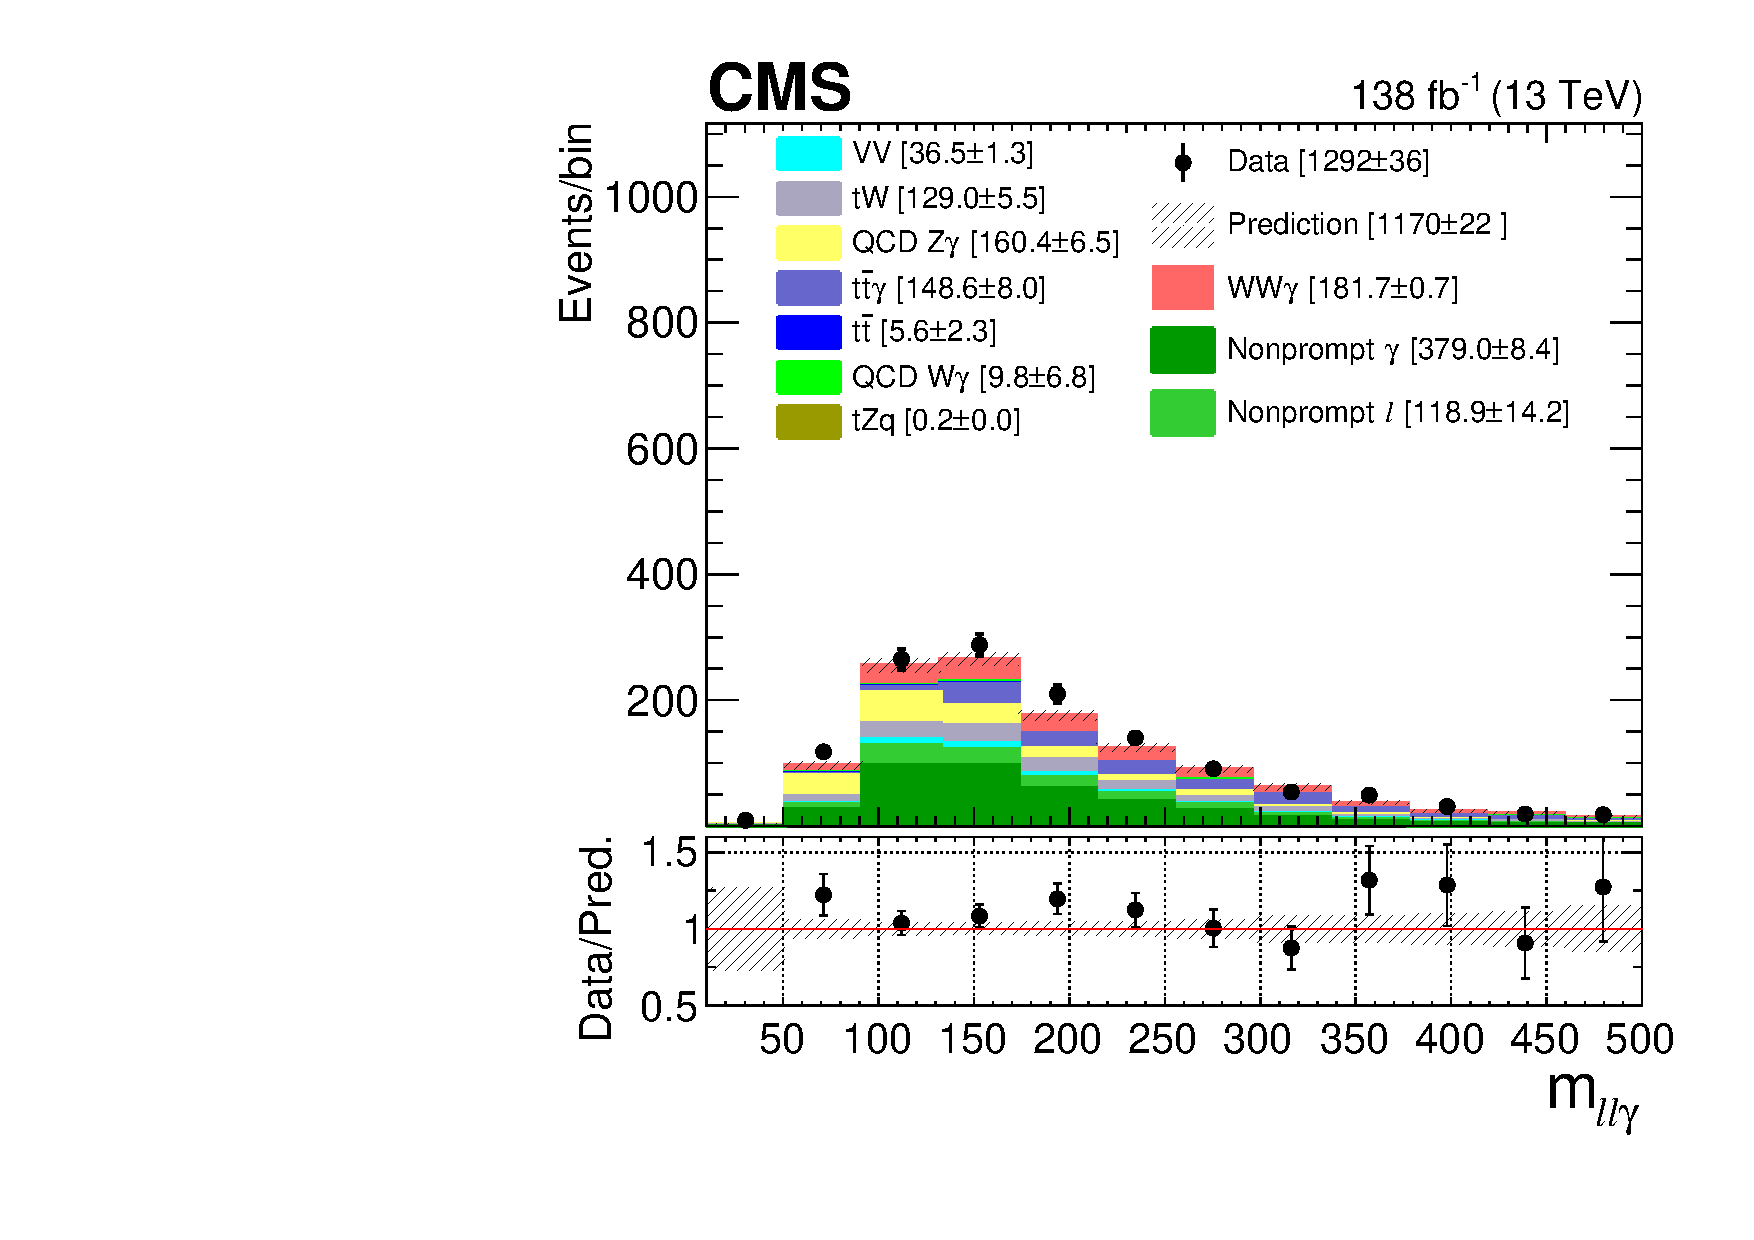
\includegraphics[width=0.48\textwidth]{unblind_SRCR/SR_prefit/can_mllg_emu.pdf}
      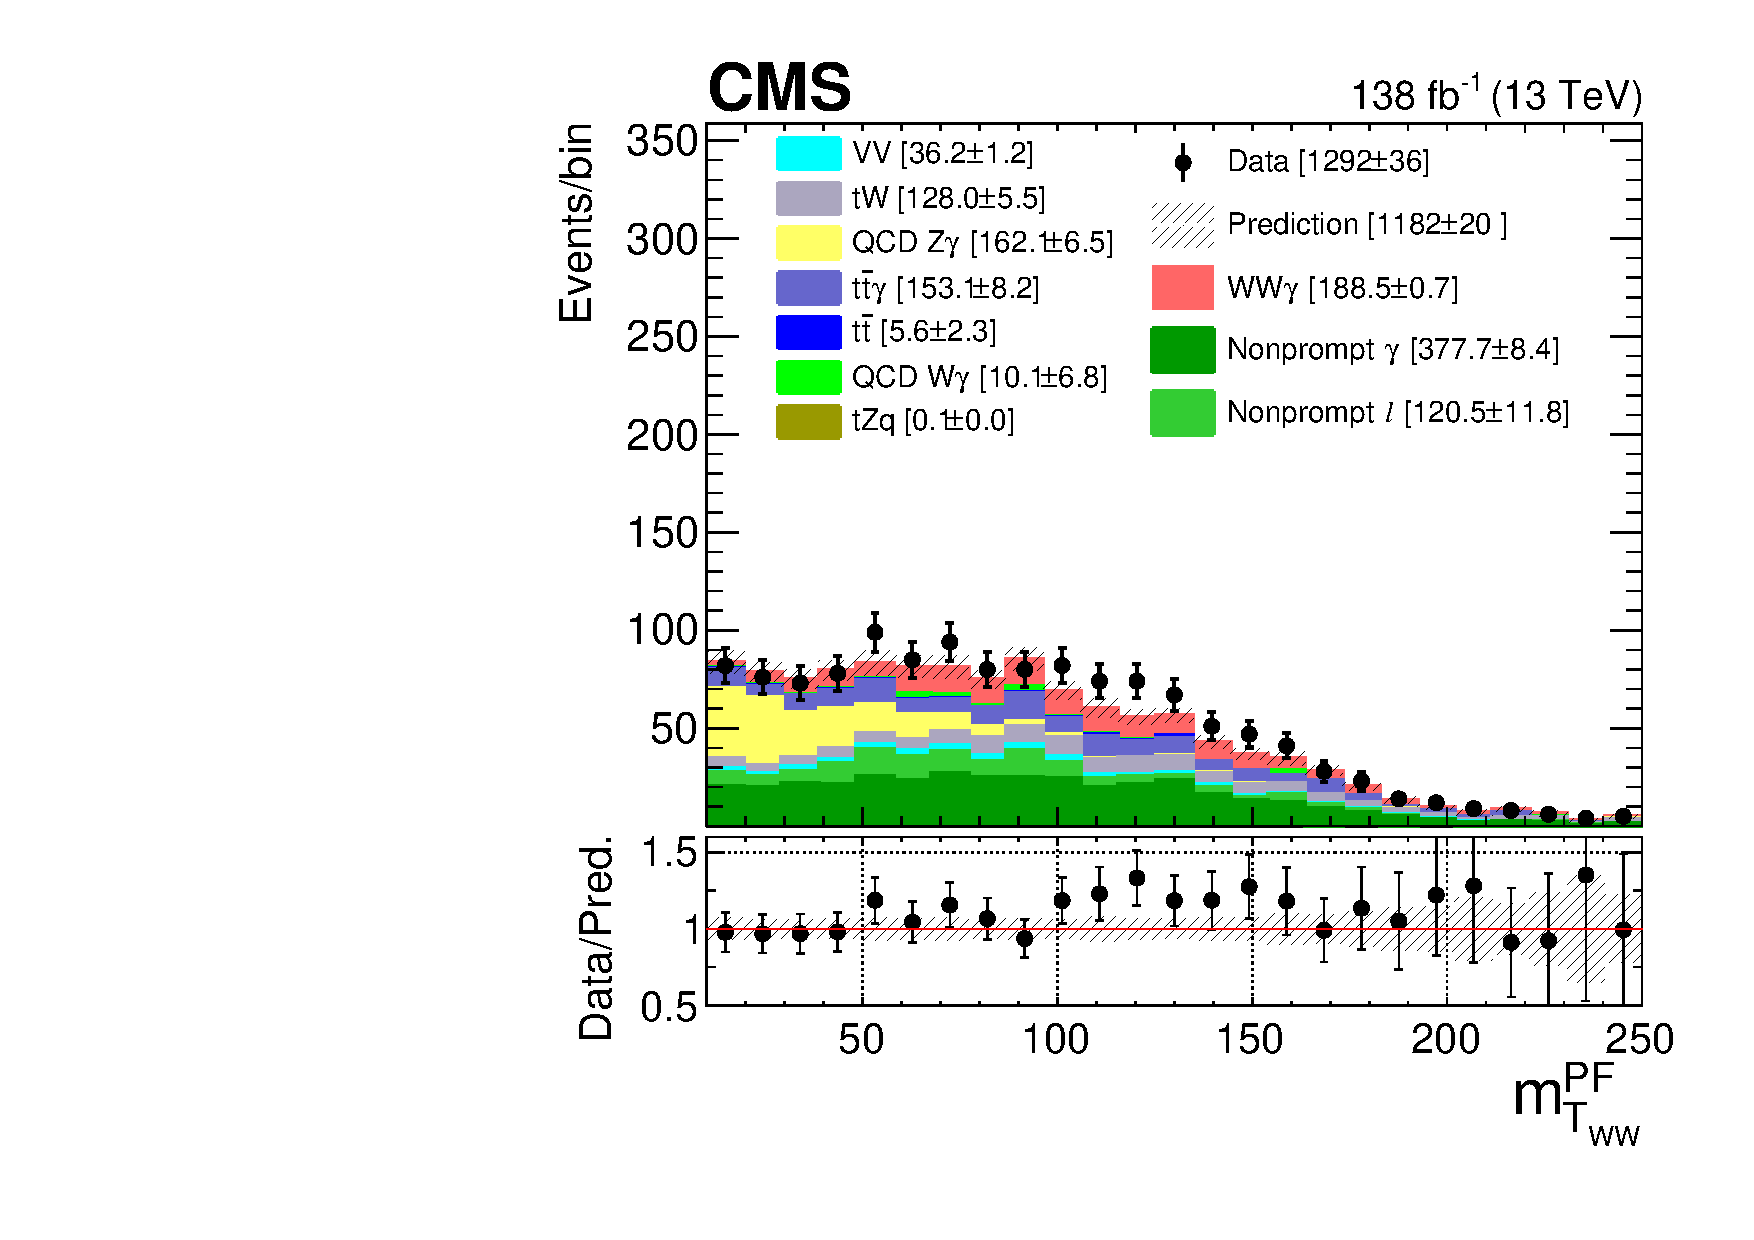
\includegraphics[width=0.48\textwidth]{unblind_SRCR/SR_prefit/can_mT_pf_emu.pdf}
      
    \caption{The pre-fit distributions of the invariant mass of the $\PW\PW\Pgg$ system (left) and the transverse mass of the $\PW\PW$ system (right) after the signal region selection. The shaded band represents the statistical uncertainty.}
        \label{fig:plots_WWgammarun2}
    \end{center}
\end{figure}

\begin{table}[!ht]
\centering
\caption{The expected and observed number of events in the control regions of the Top$\gamma$ CR and SS$\PW\PW\gamma$ and signal region.}
\begin{scotch}{lccc}
\hline
Process & Signal region & SSWW$\gamma$ CR & Top$\gamma$ CR \\
\hline
\textsc{QCD} $\PZ\gamma$ & 164.1$\pm$6.5   & 0.5$\pm$0.8 & 10.6$\pm$2.2  \\
\textsc{QCD} $\PW\gamma$ & 10.1$\pm$6.8  & 14.1$\pm$3.8  & 2.2$\pm$2.6 \\
t($\bar{\rm{t}}$)$\PW$  & 131.0$\pm$5.5  & 0.6$\pm$0.3  & 372.4$\pm$8.8  \\
\textsc{VV} & 36.9$\pm$1.3 & 24.9$\pm$1.0 & 2.0$\pm$0.3 \\
$\ttbar\gamma$ & 157.9$\pm$8.4  & 2.0$\pm$0.7  & 1345.2$\pm$25.7\\
 $\ttbar$ (FSR) & 5.6$\pm$2.3  & 0.0$\pm$0.0  & 619.5$\pm$30.0\\
t$\PZ$q & 0.2$\pm$0.0  & 0.1$\pm$0.0  & 0.6$\pm$0.1\\
Nonprompt $\gamma$ & 380.7$\pm$8.5  & 18.8$\pm$1.9  & 745.1$\pm$12.8\\
Nonprompt $\ell$ & 123.2$\pm$17.1  & 194.3$\pm$7.4  & 38.5$\pm$8.5\\
$\PW\PW\gamma$ & 195.5$\pm$0.7  & 0.9$\pm$0.1  & 9.6$\pm$0.2\\[2pt]
\hline
Expected & 1208$\pm$24  & 256$\pm$9  & 3143$\pm$43\\
Observed & 1330$\pm$26  & 263$\pm$16 & 3287$\pm$57 \\
\hline
\end{scotch}
\label{tab:yields}
\end{table}

\begin{figure}[htp]
    \begin{center}
      
      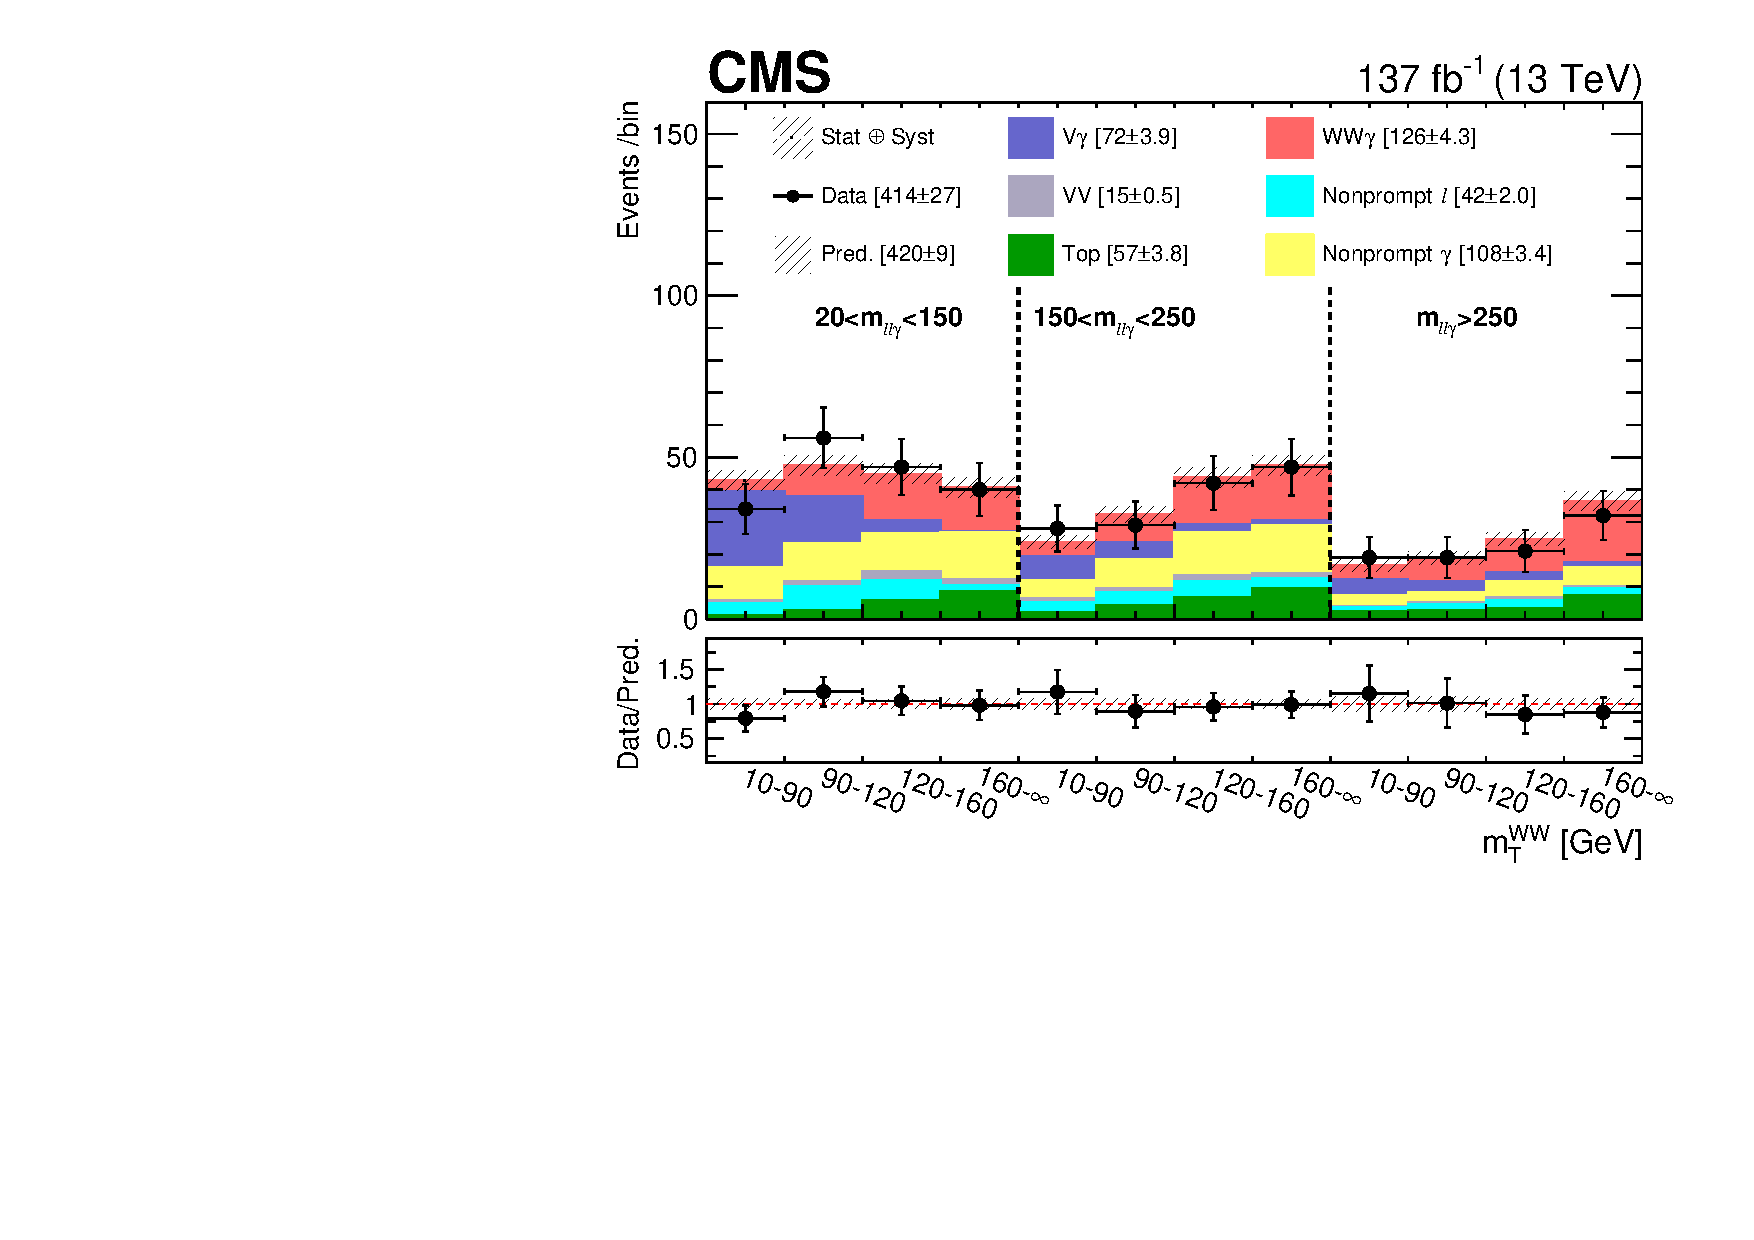
\includegraphics[width=0.48\textwidth]{unblind_SRCR/2D_fit/aa_0jetsrun2.pdf}
      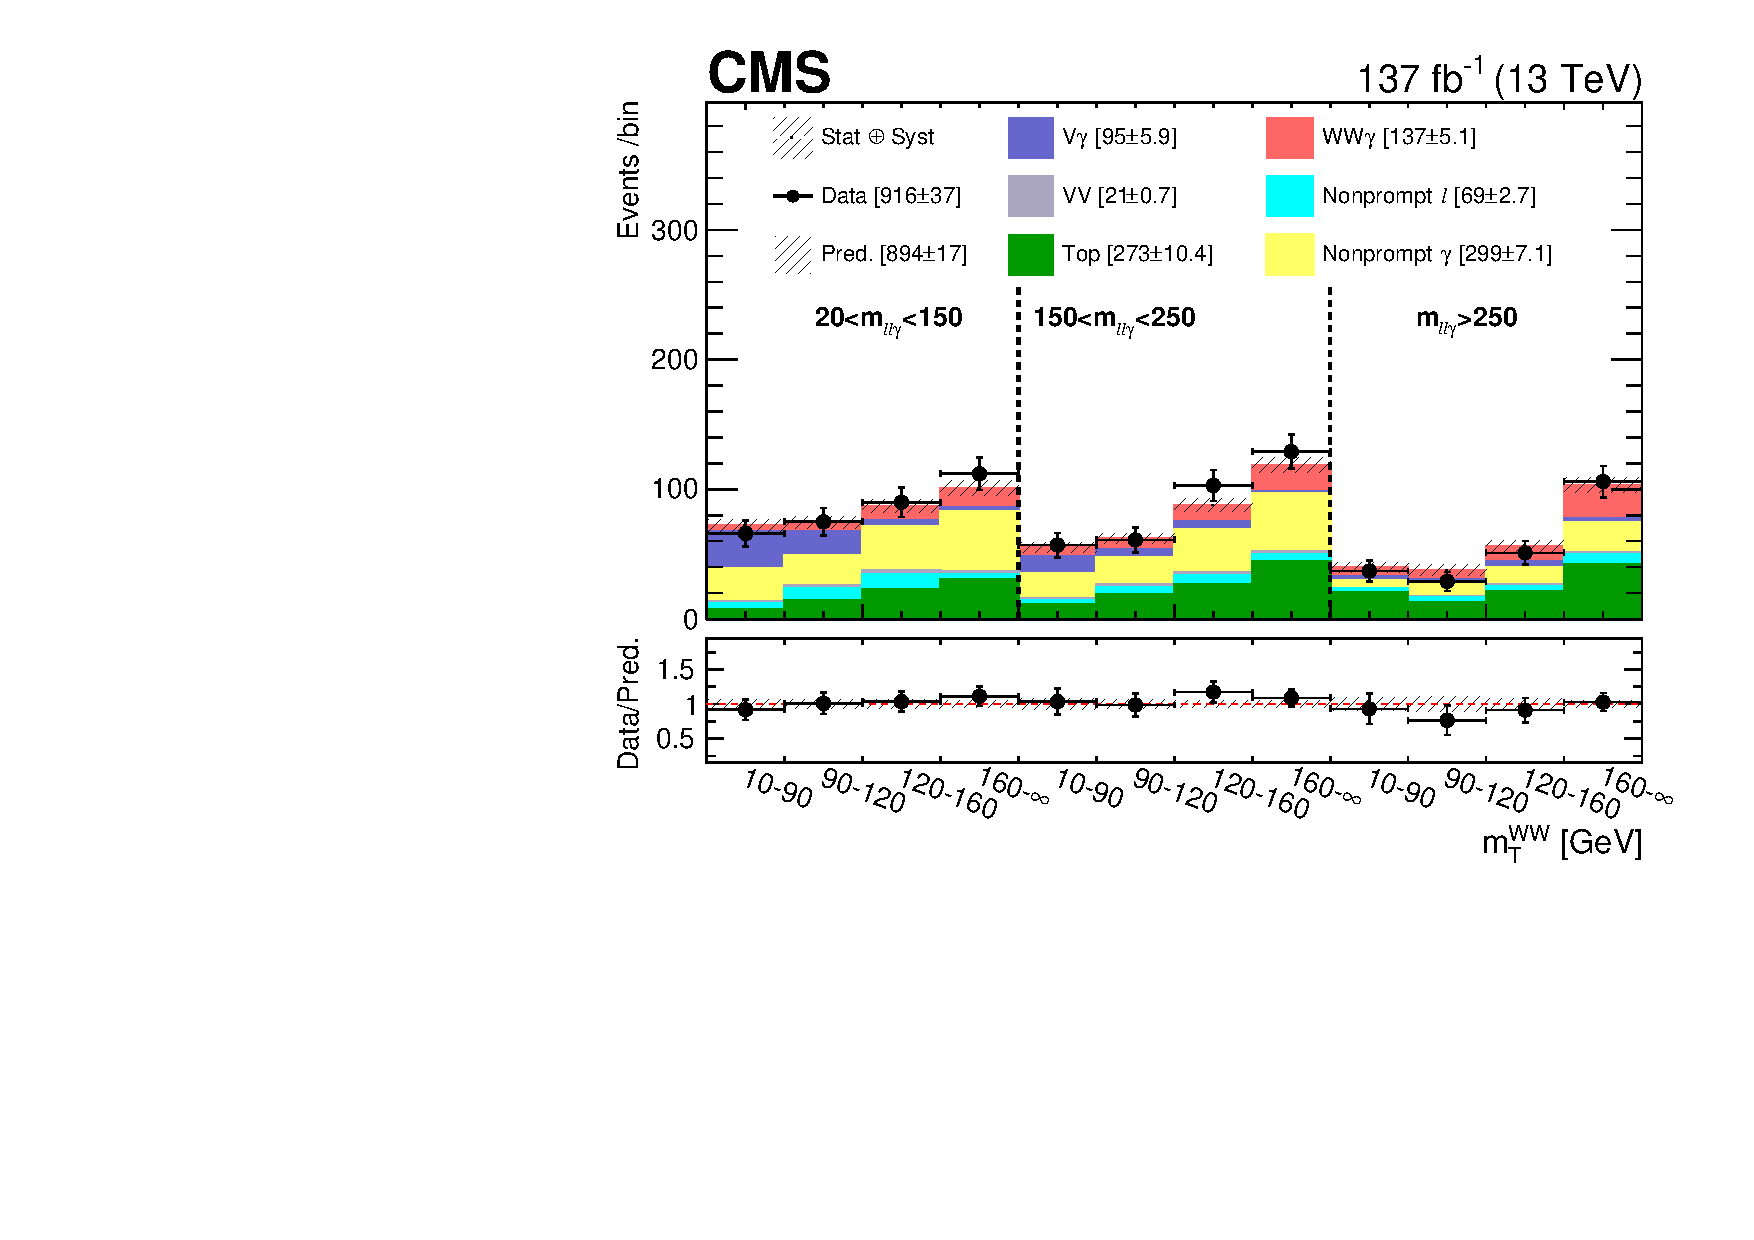
\includegraphics[width=0.48\textwidth]{unblind_SRCR/2D_fit/aa_1morejetsrun2.pdf}
    \caption{The post-fit 2D $\mTWW$-$\mllg$ distributions used for the significance measurement. The data are compared to the signal and background in the predictions. The black points with error bars represent the data and their statistical+systematic uncertainties, whereas the hatched bands represent the total uncertainties of the predictions.}
        \label{fig:2dfitrun2}
    \end{center}
\end{figure}

Various sources of systematic uncertainty are considered in the fit as nuisance parameters subject to log-normal constraints. Experimental sources of systematic uncertainty include the jet energy scale and resolution, which affect the $\ptvecmiss$, the lepton and photon identification efficiencies, the lepton trigger and b-tag efficiencies, the pileup modelling, the integrated luminosity measurement, the statistical power of our simulated samples and data control regions, and the nonprompt photon and nonprompt lepton background estimation methods. Theoretical sources of systematic uncertainty include the renormalization and factorization of QCD scales and PDFs. The renormalization and factorization of QCD scales are varied by factors of $2$ and $1/2$, excluding the (2,1/2) and (1/2,2) cases, and the envelope of these variations is taken as the uncertainty. The systematic uncertainty due to the PDFs is calculated using the members of the PDF4LHC15\_nnlo\_30\_pdfas PDF set following the PDF4LHC prescription for a Hessian PDF set~\cite{Butterworth_2016,Harland_Lang_2015,Ball_2015,PhysRevD.93.033006}. The uncertainties in the pileup modelling and the renormalization and factorization have the largest impact on the measurement.

A fiducial region is defined by applying the signal region selection at the particle level except for the requirement that the events contain no b-jets or additional lepton. The signal strength is extracted from a binned maximum likelihood fit from two-dimensional (2D) distributions in bins of $\mTWW$ and $\mllg$, where the likelihood function is the product of a Poisson probability density function for each bin. A simultaneous fit in both signal and control regions is used for our results leading to the observed and expected signal strengths of $\mu^{\text{obs.}}_{\text{combined}}=1.31 \pm 0.17 \stat \pm 0.21 \syst$ and $\mu^{\text{exp.}}_{\text{combined}}=1.0 \pm 0.16 \stat \pm 0.18 \syst$. The theoretical prediction for the fiducial cross section is $4.61 \pm 0.34 \text{ (scale)} \pm 0.05 \text{ (PDF)} \unit{fb}$ based on the NLO QCD \MGvATNLO simulation. The measured cross section from the simultaneous fit with the uncertainties divided into statistical, experimental, and theoretical components is $\sigma = 6.04 \pm 1.69 \unit{fb} =6.04 \pm 1.03 \stat \pm 0.97 \syst \pm 0.85 \thy \unit{fb}$.

Next, we search for $\PH\gamma$ production with modified Higgs boson couplings to light quarks. The selection for the Higgs search is similar to the EW signal selection, but targets the Higgs characteristics by requiring $\dphill<2.5$, $\drll<2.3$, and $\Delta R_{l\gamma} >0.8$. As strong power of the $\Delta R_{\ell\ell}$, the profile likelihood ratio test statistic~\cite{CMS-NOTE-2011-005} is built in bins of $\Delta R_{\ell\ell}$ and $\mTH$, where $\Delta R_{\ell\ell}$ and $\mTH$ are divided into bins [0.5,1.8,2.0,2.3) and [0, $\infty$), respectively. The expected and observed $\PH\gamma$ cross sections at 95\% confidence level are shown in Table~\ref{tab:Limits Hgamma1}. Under the “flat direction” theoretical assumption~\cite{PhysRevD.103.095023} that all other SM $\kappa$ scale as $\kappa_{\PH}$, the results can be reinterpreted to the Higgs to light quarks Yukawa couplings.%For these light quarks, the limits are shown in Table~\ref{tab:Limits Hgamma2}.

\begin{table}[h]
\centering
\caption{Upper limits on the cross section and reinterpreted Yukawa couplings limits for $\PH\gamma$ production initiated by light quarks.}
\begin{scotch}{cccc}
\hline
Process  & $\sigma_{\text{up}}$ \unit{pb} exp.(obs.)   & Yukawa couplings limits exp.(obs.)\\\hline
$\PQu \overline{\PQu} > \PH+\gamma > \Pe\mu\gamma$  & 0.0811 (0.1022)  & $ \lvert\kappa_{\PQu}\rvert  \leq $12862.2 (15772.2)\\[2pt]
$\PQd \overline{\PQd} > \PH+\gamma> \Pe\mu\gamma$   & 0.0663 (0.0820)  & $ \lvert\kappa_{\PQd}\rvert  \leq $14200.8 (17227.2)\\[2pt]
$\PQs \overline{\PQs} > \PH+\gamma> \Pe\mu\gamma$   & 0.0583(0.0811)  & $ \lvert\kappa_{\PQs}\rvert  \leq $1309.5(1670.34)\\[2pt]
$\PQc \overline{\PQc} > \PH+\gamma> \Pe\mu\gamma$   & 0.0667(0.0870)  & $ \lvert\kappa_{\PQc}\rvert  \leq $112.3(195.6)\\
\end{scotch}
    \label{tab:Limits Hgamma1}
\end{table}

\iffalse
\begin{table}[h]
\centering
\caption{Expected limits on the $\PQu$, $\PQd$, $\PQs$, and  $\PQc$ quark Yukawa couplings in three frameworks.}
\begin{scotch}{c c c c}
\hline
$\kappa$/interpretation &  Quadratic (95\%CL) & BR variation (68\%CL)  & Flat Direction (95\%CL)\\[2pt]
$\kappa_{\PQu}$   & -9894.0,9894.0       & -9467.2 , 9467.2      & -13890.4, 13890.4\\[2pt]
$\kappa_{\PQd}$  & -10534.2,   10534.2 & -10864.0,10864.0       & -15364.8   ,   15364.8\\[2pt]
$\kappa_{\PQs}$  & -873.0 ,   873.0 & -       & -873.0 ,   873.0  \\[2pt]
$\kappa_{\PQc}$  & -95.095  ,   95.095 & -   & -94.86  ,   94.86      \\[2pt]
\end{scotch}
    \label{tab:Limits Hgamma2}
\end{table}
\fi
In summary, this letter reports the first observation of $\PW\PW\gamma$ production in proton-proton collisions at a center-of-mass energy of 13\TeV, with an integrated luminosity of 138\fbinv, collected by the CMS experiment at the LHC in 2016--2018. The measured fiducial cross section for $\PW\PW\gamma$ is $6.04 \pm 1.69 \unit{fb}$, in good agreement with the next-to-leading order QCD prediction. \iffalse Exclusion limits on anomalous quartic gauge couplings are derived at 95\% confidence level in terms of the dimension-8 effective field theory operators.\fi 
A search for the associated production of a Higgs boson and a photon was also performed using the Higgs boson decay to $\PW^{+}\PW^{-}$. A set of 95\% confidence level limits on the Higgs couplings with light quarks were reported, including some of the most stringent to date.

\begin{acknowledgments}
We congratulate our colleagues in the CERN accelerator departments for the excellent performance of the LHC and thank the technical and administrative staffs at CERN and at other CMS institutes for their contributions to the success of the CMS effort. In addition, we gratefully acknowledge the computing centers and personnel of the Worldwide LHC Computing Grid for delivering so effectively the computing infrastructure essential to our analyses. Finally, we acknowledge the enduring support for the construction and operation of the LHC and the CMS detector provided by the following funding agencies: BMBWF and FWF (Austria); FNRS and FWO (Belgium); CNPq, CAPES, FAPERJ, FAPERGS, and FAPESP (Brazil); MES (Bulgaria); CERN; CAS, MoST, and NSFC (China); COLCIENCIAS (Colombia); MSES and CSF (Croatia); RPF (Cyprus); SENESCYT (Ecuador); MoER, ERC IUT, PUT and ERDF (Estonia); Academy of Finland, MEC, and HIP (Finland); CEA and CNRS/IN2P3 (France); BMBF, DFG, and HGF (Germany); GSRT (Greece); NKFIA (Hungary); DAE and DST (India); IPM (Iran); SFI (Ireland); INFN (Italy); MSIP and NRF (Republic of Korea); MES (Latvia); LAS (Lithuania); MOE and UM (Malaysia); BUAP, CINVESTAV, CONACYT, LNS, SEP, and UASLP-FAI (Mexico); MOS (Montenegro); MBIE (New Zealand); PAEC (Pakistan); MSHE and NSC (Poland); FCT (Portugal); JINR (Dubna); MON, RosAtom, RAS, RFBR, and NRC KI (Russia); MESTD (Serbia); SEIDI, CPAN, PCTI, and FEDER (Spain); MOSTR (Sri Lanka); Swiss Funding Agencies (Switzerland); MST (Taipei); ThEPCenter, IPST, STAR, and NSTDA (Thailand); TUBITAK and TAEK (Turkey); NASU (Ukraine); STFC (United Kingdom); DOE and NSF (USA). 
\end{acknowledgments}

\bibliography{auto_generated}


